\documentclass[12pt]{article}
\usepackage{dicas}

\def\tam{0.5}

\title{Dicas para Concurso de Professor}
\author{Geraldo Xexéo}
\affil{\url{xexeo@ufrj.br} \\
\url{http://xexeo.net}}
\date{\ccbyncsa\  - \today}

\begin{document}


\maketitle

\begin{abstract}
    Este documento apresenta dicas para provas de aula de concurso para universidades públicas, que devem ser usadas tanto em concursos para professor adjunto quanto para professor substituto.
\end{abstract}

\section{Dicas Gerais}

Em geral, as dicas gerais mais importantes são sobre sua imagem.

Vá bem vestido, com calça e roupa social, ou traje feminino equivalente, possivelmente com um blazer se estiver mais frio. Lembre que o ambiente universitário é informal, então não vá de terno, a não ser que a área se vista normalmente assim, por exemplo em um curso de direito. Use sapatos, cinto, etc. Barba e cabelos aparados, não pareça um cientista louco. Lembre-se que existe preconceito e que a ``primeira impressão é a que fica''.

Use um português correto, evite ao máximo as gírias e considere palavrões e blasfêmia como erros graves. Não apresente opiniões políticas ou religiosas, se mantenha no nível técnico. Fale de maneira clara, sempre de frente para a banca, evite vícios de linguagem, como repetir "ok" no final das frases. Se for usar termos em outras línguas investigue como devem ser pronunciados corretamente, e não confie na pronúncia de conhecidos.




Chegue adiantado, isto é, não basta chegar no horário. Prepare-se para esperar por um membro da banca atrasado. Leve água e um possível lanche, se achar que pode demorar muito. Não demonstre irritação com problemas de controle de tempo no concurso, ou problemas em equipamentos ou falta de materiais, porque são comuns. Caso se sinta prejudicado por um desses problemas, peça para anotarem na ata, mas mostre disposição para resolvê-los, ou esperar sua solução.

Apresente todos os seus documentos organizados, em pastas, com índice e na ordem de avaliação do edital e da contagem de pontos do concurso. Indique a quantidade de itens que estão sendo apresentados para cada pontuação prevista.

\section{Dicas para a Prova Escrita}

Atenção, para a prova escrita \textbf{leve um relógio} simples, que claramente não permita se comunicar com ninguém. O controle de tempo é muito importante. Lembre-se que é certo que  não possa usar um \textit{smartphone}.

Leve lápis ou lapiseira, apontador, borracha, mais de uma caneta preta, mais de uma caneta azul, régua e outros materiais que podem ser necessário em sua área. Normalmente não há problema em levar gabarito para fluxogramas ou outro tipo de diagrama (\autoref{fig:gabarito}).

\begin{figure}
    \centering
    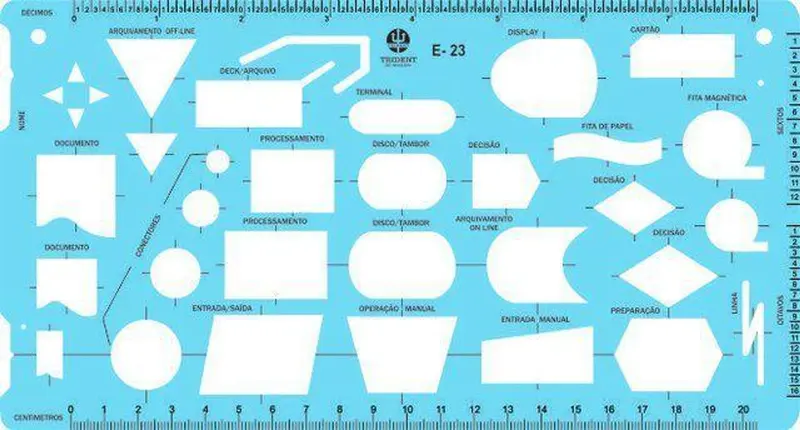
\includegraphics[width=0.6\textwidth]{gabaritofluxograma.png}
    \caption{Gabarito para fluxograma, ainda encontrado a venda.}
    \label{fig:gabarito}
\end{figure}


Alguns concursos permitem ou até demandam o uso de calculadoras, porém pode haver limites no poder computacional ou no poder de comunicação das mesmas. Calculadoras para as quatro operações alimentadas por energia luminosa podem ser muito baratas. Calculadoras científicas não programáveis tem também preços razoáveis. No caso de uso de calculadoras, preste muita atenção ao que o edital permite ou não permite.

Preste atenção à qualidade da letra. Letras bonitas levam a uma boa avaliação. A seguir, na organização do texto, com seções, parágrafos e frases bem delineadas. Mantenha a folha limpa e evite rasuras.

A prova escrita deve ter mais de uma questão e você deve dividir o tempo de forma igual para todas as questões.
Divida o tempo em planejamento, execução e se houver tempo suficiente rascunho, e o tempo de passar a limpo.

Deixe um tempo para uma pequena revisão. Faça ensaios para descobrir quanto tempo leva para escrever uma certa quantidade de texto e decorar o máximo possível respostas para questões dissertativas genéricas sobre os pontos da prova.

Correções a textos feitos com caneta devem ser feitas com um risco simples sobre o texto, \st{assim}.. Concursos não devem permitir o uso de tinta corretora, e não devem ser feitos rabiscos muito grossos. Uma vantagem do risco simples é que se for algo correto, a banca pode resolver considerar, ou pelo menos haverá um viés psicológico positivo, mas se for errado, nunca descontará ponto.

Antes de começar a escrever faça um plano no rascunho. Eu recomendo começar com um mapa mental e depois uma itemização. Ao escrever siga os itens planejados, porém não há problema em estender um ou trocar alguma coisa, se você mantiver o tempo controlado e parar para pensar sobre o que está fazendo em relação ao seu plano. Lembre que tudo deve estar planejado no tempo.

Se você tem que dar a resposta com um texto que vai criar na hora, deve guardar um tempo para uma revisão final. Havendo necessidade de correções, corte com riscos simples (de preferência use a régua) e insira com símbolos claros que levem a "notas de fim de texto", numeradas e claramente separadas.

Já vi provas onde o espaço é delimitado, nesse caso vale mais a  pena fazer um rascunho do que nas provas onde o espaço é livre.

No caso de espaço livre para as questões, saiba o seu ritmo. Por exemplo, nas provas em que fiz me preparei para responder uma questão com aproximadamente 4 páginas de papel almaço (1 folha), em um hora, incluindo planejamento, rascunho e escrita.

Normalmente os concursos são feitos em papel almaço, pautado, se não houver pauta, pode faça uma pauta a lápis usando a régua.

A maioria das provas que vi eram questões dissertativas sobre um tópico. Porém, é possível que seja dado um problema para resolver.

\subsection{Questões Dissertativas}

Nas questões dissertativas, é comum pedir "disserte sobre o ponto", onde o ponto é algum dos apontados na ementa do concurso.
É sempre bom se preparar para esse tipo de prova criando um texto padrão para responder uma pergunta desse tipo para cada ponto.
É possível então treinar para responder a questão no tempo hábil.

Sempre comece do mais geral para o mais específico.

Em questões desse tipo é importante usar a técnica 5W2H. Comece explicando \textbf{o que} é o tópico, com uma definição formal e uma explicação que a torne mais clara. Depois trabalhe sobre o \textbf{porquê}, discutindo motivação, razões por que é usado. O próximo tema é \textbf{como}, explicando como ele é feito. \textbf{Onde} é usado, e \textbf{quando} é usado, \textbf{quem usa} e \textbf{qual o seu custo} (por exemplo, complexidade computacional) também são dados importantes.

É importante ter uma visão histórica do tema, autores mais importantes, se possível sabendo a referência completa. Além disso, sempre faça diagramas, desenhos, forneça as fórmulas e dê um exemplo detalhado de uso, com explicação.

Se houver alguma notação gráfica relevante ao tema, como UML ou Entidades e Relacionamentos, faça uma tabela indicando o significado de cada desenho e exemplos diferentes com possibilidades de uso da notação.

Listas ou enumeração são bons mecanismos, mas devem ser usados com parcimônia, pois ocupam espaço e não têm fluxo de leitura. Não se esqueça que em alguns casos é necessário terminá-las com indicações de que elas são infinitas, ou muito grandes, e você só está dando exemplo. Além disso, quando se fala de taxonomias, como de tipo de jogos, sempre é possível que existam soluções híbridas, que devem ser citadas no final. No caso de lista que possuam exemplos, não esqueça de citá-los.

Sempre que possível, forneça um exemplo de uso. Por exemplo, se o tema for "Modelo X", explique tudo com o 5W2H em mente e depois faça um exemplo de uma modelagem simples com o exemplo que mostre algumas particularidades.

Divida seu texto em tópicos, principalmente se houver uma lista de itens na resposta, deixando claro que parte do seu texto responde a que parte da pergunta.

É bom também criar uma introdução que contextualize a resposta e uma conclusão.

Se possível, coloque as referências. Faz diferença positiva apresentar um texto referenciado.

Lembre-se que é importante se manter no tema.

\subsection{Questões do tipo problema para resolver}

No caso de questões do tipo problema a resolver, havendo espaço, não se esqueça de antes de resolver fazer um modelo do problema e da solução e indicar todas as fórmulas e algoritmos que vão ser usados.
Depois disso feito, mostre que valores as variáveis assumem no modelo, mostre a memória de cálculo e a solução final.

Lembre-se que é fácil errar em cálculos, então aproveite para mostrar seus conhecimentos, porém sem fugir do tema.

Havendo tempo e espaço suficiente em questões desse tipo, é possível mostrar como as fórmulas usadas são encontradas, analisar casos mais gerais ou específicos, sempre dentro do tema da questão e dentro do equilíbrio de tempo entre as questões.

\section{Dicas Para a Prova de Aula}

A prova de aula é uma \textbf{aula}, que deve ser dada para a banca como se ela fosse dada para uma turma típica da  da instituição para a qual você concorre, mais provável que no nível de graduação. Na prática, é quase um teatro\footnote{Aviso porque já vi um candidato dar uma palestra de como seria a sua aula, e isso levou a uma nota muito baixa.}.

É muito importante considerar que  a aula é dada para pessoas com um nível específico de conhecimento. Normalmente, o nível é de graduação, sendo que a aula deve ser dada como se para alunos que não sabem o tema. A linguagem deve ser adaptada e é necessário tomar cuidado com o que consideramos que os ``alunos'' sabem. Por isso, é importante, no início da aula, deixar clara sua premissa sobre o conhecimento dos alunos. Isso deve ser feito usando a própria aula, como se lembrando aos alunos o que eles aprenderam antes, no próprio curso ou possivelmente em outro curso.

Tente manter o nível de exigência para conhecimentos prévios baixo. Por exemplo, se for dar exemplos com linguagem de programação, use apenas uma linguagem\footnote{A não ser que o tema leve a necessidade de comparar linguagens}, e a mais simples possível (Python provavelmente, hoje em dia, se não houver necessidade de declarar tipos).

Você deve usar exatamente o tempo destinado à prova de aula, nem mais, nem menos. Para isso, o ideal é preparar uma aula um pouco menor, porém com exercícios ou outras atividades no fim, que possam ser feitos ou ser passadas rapidamente como ``dever de casa''.
Desse jeito, você pode atrasar um pouco sem se preocupar muito, utilizando essa margem para explicações e exemplos melhores que descobriu ou lembrou naquele instante. Isso será compensado mais tarde, reduzindo a atenção dada aos exercícios.
Por outro lado, você também pode usar esses exercícios para usar um tempo que tenha sobrado. Isto pode ser feito dando o exercício ou dando dicas para resolvê-lo.

Durante a aula, pergunte se alguém tem dúvida (ninguém vai responder). Além disso, você pode preparar uma ``dúvida'' e dizer algo ``Como ninguém tem dúvida, eu tenho uma'' e fazer um esclarecimento mais profundo\footnote{Lembre-se, é um teatro!}.


A aula deve estar no contexto de um curso. Você deve procurar a ementa do curso para o qual estaria dando aula, dentro do departamento para o qual faz o concurso, e, no início da aula, contextualizar a mesma dentro de um curso imaginário que cumpra essa ementa. Por exemplo, você pode mostrar a lista de assuntos do curso e mostrar em que aula está. Deve também falar um pouco sobre a última aula e como ela e a aula atual se relacionam. Também deve, ao final da aula, fazer uma pequena citação de qual será o próximo assunto, de preferência com a ligação de como o assunto da aula será usado.

O \textbf{português} utilizado será determinante na sua pontuação.
Erros de português no material impresso são graves, e erros de fala são normalmente percebidos e causam perda de pontos.
Muito cuidado com a concordância verbal e com defeitos de linguagem que sabemos que temos, mas não nos preocupamos na fala coloquial.
Pessoas de outros estados, diferentes do local do concurso, devem tomar cuidado com expressões de seu local de origem que não serão compreendidas pela banca.

Se você já deu aulas, deve tentar fazer ou simular tudo que faz com seus alunos normalmente, principalmente o que tem sucesso, e o que gostaria de fazer.
Por exemplo, criar um \textit{Moodle} ou um \textit{Google Classroom} para a turma.
Na aula, você deve então indicar em que parte do \textit{site} está sua aula, como os alunos podem baixar e que exercícios devem fazer ou entregar.

A prova de aula, como diz o nome, é sobre como você dá aula.
Use sua experiência. Não se preocupe em estar apresentando a aula para uma banca de professores reconhecidos ou exigentes.
Não é uma apresentação de trabalho em congresso, você deve dar a aula  como se fosse para sua turma, porém com um cuidado adicional de não ser tão informal ao ponto de cometer erros de comportamento ou de português.

Ao preparar a aula, lembre-se que a banca não só já conhece o assunto como pode ser especialista nele, mas os supostos alunos, não. A banca leva isso em consideração.
Eu recomendo procurar fontes sólidas, ter cuidado com a profundidade em que o tema é abordado e buscar a facilitação do aprendizado, através de exemplos e exercícios.
O objetivo não é demonstrar seu conhecimento sobre o tema, o que acontece na prova escrita, mas sim demonstrar sua capacidade de ensinar o tema.

Se o tema for muito amplo, você tem duas opções: dar uma aula introdutória ou escolher um sub-tema.
A validade de escolher um sub-tema pode ser perguntada a banca, que pode ou não responder.
Se a banca não responder, sugiro escolher a aula introdutória.
Nessa aula, no final você deve indicar como as próximas aulas vão se aprofundar no tema.

Não se esqueça de trazer exemplos reais, e aplicações do seu tema a vida real.



\subsection{Material para a aula}

Você deve tentar levar todo o material possível para a aula.

Caso vá usar um computador para fazer a apresentação e possua um notebook, deve tentar apresentar com seu equipamento, já que isso diminuirá a chance de problemas por não saber onde está algum software necessário ou com versões do mesmo.

Se pretende usar giz ou quadro branco, deve levar seus kits coloridos e apagadores, pois não necessariamente terá todo o material que desejam disponível na hora.


Sempre traga a aula, em vários formatos, em um drive USB, caso seu computador, ou outro, falhe, ou a rede não funcione. Não confie na rede!

Se não for usar seu computador, salve sua aula não só no formato original, mas também em formatos alternativos.
Não deixe de ter a apresentação em formato .pdf, que transita bem entre os vários sistemas operacionais.

Não esqueça de, ao criar os arquivos .ppt, .pptx ou .pdf, incluir as fontes dentro deles.

Se possível, leve um ``passador de slides'', aquele controle remoto que permite passar os slides à distância.

\subsection{Slides}

Recomendo o uso de slides, como chamarei aqui a apresentação tipicamente feita com \textit{Power Point}.
Eles devem estar incluídos na lista de recursos didáticos e devem ser entregues, de forma impressa, para a banca, representando o fato de eles estarem disponíveis em algum site ou \textit{Course Management System - CMS}, como o \textit{Moodle}.

A média de slides como os que apresento neste texto é de 2 a 3 minutos, porém alguns slides demoram muito pouco, porque são apenas marcos para indicar em que ponto da aula estamos. Muitas vezes eu considero que, entre os slides onde falo e aqueles que são só ``um flash'', como títulos de seções, realizo uma média de 1 minuto por slide.

\textbf{Todos seus slides devem estar em português}, a não ser que seja outra a exigência do concurso, o material, como um todo, deve ser original.
Tudo que não for original deve ter uma citação.
A consideração com os alunos também é avaliada, tanto quanto a suposta ``preguiça'' de não fazer o material próprio.
Não apresente um material pré-pronto, como o disponível para acompanhar um livro.
Faça o seu material, dite seu próprio ritmo.
Nada impede, porém, que se inspire em outras aulas disponíveis na rede.

O ideal seria você criar do zero todas as imagens.
Claro que algumas imagens não podem ser originais, como fotos.
Por exemplo, no slide \ref{fig:crisis} eu mostro uma caricatura original em inglês, da época da Crise do Software.
No concurso, na verdade, sempre há  margem de usar imagens de outros autores, porque o tempo é curto.
É necessário, porém, citar a fonte.

\begin{figure}[!htb]
    \centering
    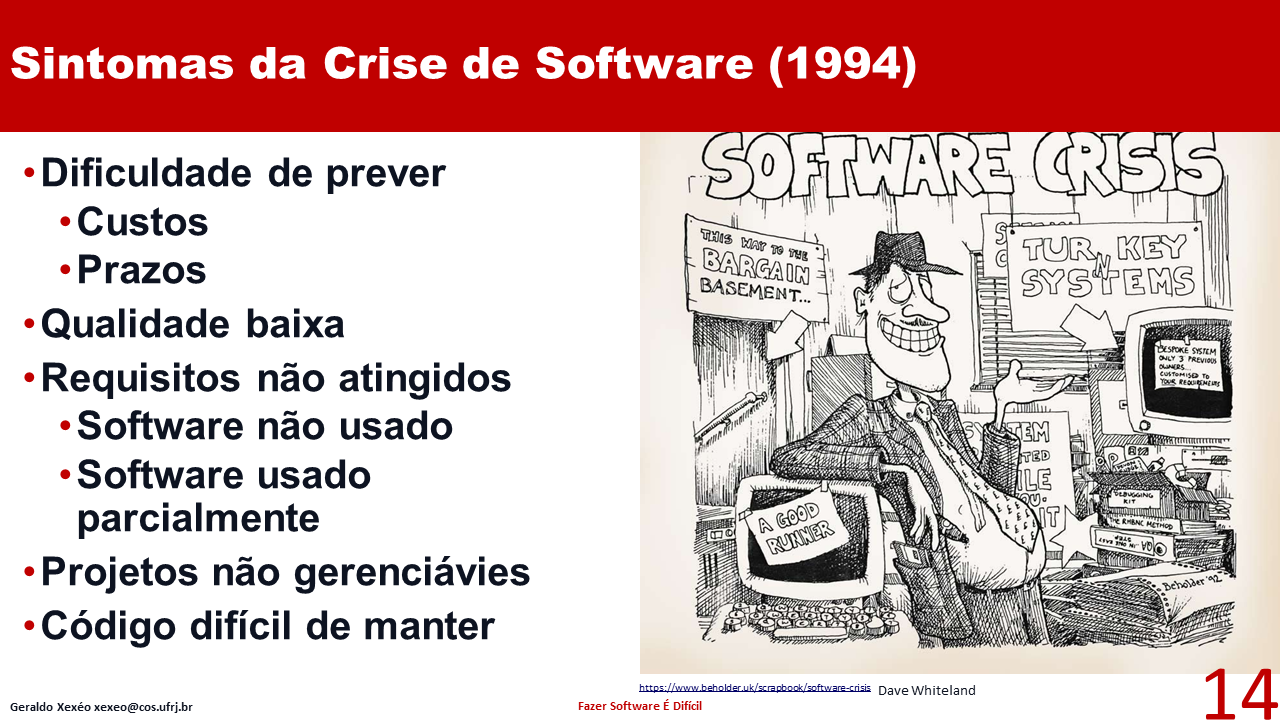
\includegraphics[width=\tam\linewidth]{imagens/crisis.png}
    \caption{Slide mostrando uma imagem original, onde a língua original é permitida.}
    \label{fig:crisis}
\end{figure}

Deve-se evitar slides que falam muito sobre algo sem mostrar como é feito.
Há algum tempo eu costumo dar \textit{spoilers} mostrando as coisas antes de explicar o que são, sobre que estou falando, mas só mostrar uma imagem no mesmo slide em que se explica algo ajuda muito.

A ideia aqui é não confundir a banca, ou os possíveis alunos, e indicar para onde estamos indo. Isso também pode ser feito com texto ou com matemática.
Por exemplo, em uma sequência de slides onde se prova um teorema ou se calcula algo podemos sempre mostrar nosso objetivo.

A Figura \ref{fig:teximag} mostra a explicação de um ator em um Diagrama de Caso de Uso sendo feita, ao mesmo tempo, de forma conceitual e gráfica. Seria ainda melhor se houvesse um pequeno exemplo de uso.

\begin{figure}[hbt]
    \centering
    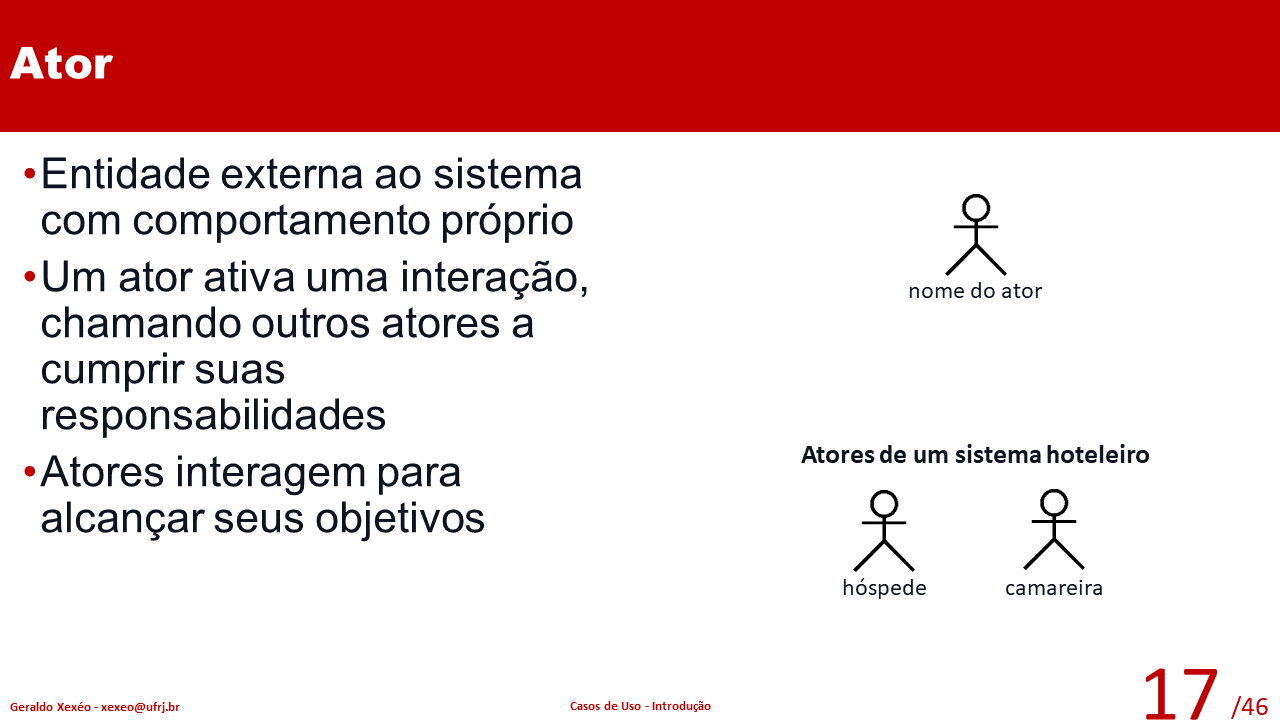
\includegraphics[width=\tam\linewidth]{imagens/slidecomimage.png}
    \caption{Slide com texto e imagem}
    \label{fig:teximag}
\end{figure}

Você, porém, \textbf{não deve usar apenas os slides ao dar a aula}, devendo também usar o quadro branco ou negro, por exemplo, para resolver um problema ou mostrar alguma ideia adicional. Esse recurso, o quadro branco ou negro, deve estar na lista de recursos. Se conseguir pensar em outros recursos, melhor.


\subsection{Regras essenciais sobre os slides}

Os slides \textbf{devem ser numerados} e conter em cada slide o número total de slides, possivelmente no formato ``slide/total'', como em ``4/40''.
Eu uso números bem grandes e recomendo usá-los\footnote{Na minha prática diária, eu muitas vezes não tenho o total de slides porque insiro e retiro slides de acordo com a evolução da aula, e o \textit{Power Point} não suporta o  total de slides automático, mas sempre tento fazer isso na mão}.

Todo slide deve ter um \textbf{título único}. Algumas pessoas gostam de usar um título de seção e um subtítulo que diz o que realmente o slide diz, mas isso faz com que cada slide pareça ser o mesmo que o outro e eu discordo dessa abordagem.
A Figura \ref{fig:coppe} mostra um slide seguindo essa regra.
A Figura \ref{fig:meio} mostra um slide que tem todas as seções identificadas em seu cabeçalho, sendo que a seção atual está com ênfase.
Nesse caso, o título principal ainda é o título do slide.
Isso pode ser feito automaticamente em alguns estilos para \texttt{beamer} no \LaTeX.




Todos os slides devem identificar a aula, o autor, incluindo o e-mail.
Eu coloco isso no rodapé, o que é realmente o lugar para colocá-los no \textit{Power Point}.
A instituição pode ser indicada através de um logo, como o slide da Figura \ref{fig:coppe}\footnote{Os slides vermelhos não têm a identificação da instituição porque são usados em mais de um curso}.

\begin{figure}[htb]
    \centering
    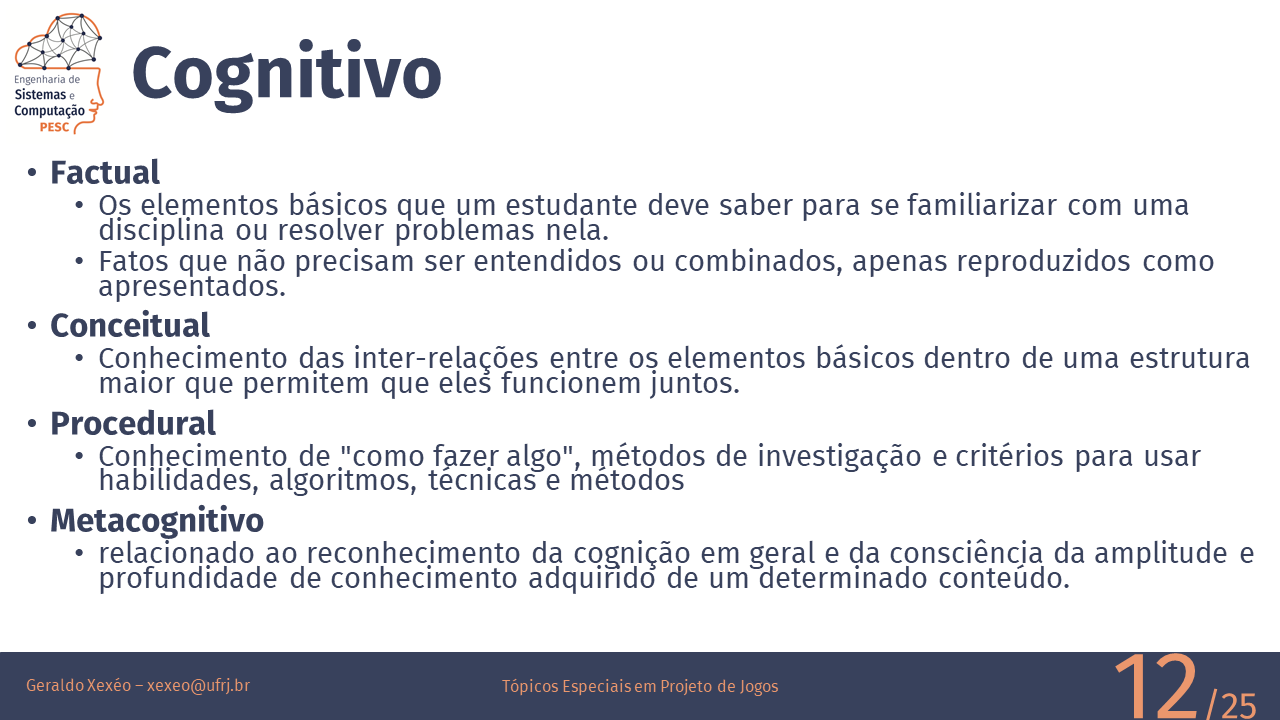
\includegraphics[width=\tam\linewidth]{imagens/slideexemplotepj.png}
    \caption{Um slide com logo, um título único, identificação, número do slide e número total de slides}
    \label{fig:coppe}
\end{figure}

Use fontes ``limpas'', não rebuscadas, e \textbf{sem-serifa}\footnote{Serifas são as pontinhas que existem em algumas fontes. Elas estão bem visíveis no S da palavra ``slides'' desta seção.}, como Arial ou Calibri, e \textbf{corpos grandes}, 32 pts, por exemplo.
Os slides das Figuras \ref{fig:coppe} e \ref{fig:teximag} seguem essa regra.
Já o slide da figura \ref{fig:formulas} usa um tamanho menor para o corpo das fórmulas.
Lembre que a banca, ao invés dos alunos, é mais velha e pode ter dificuldades de visão.

A melhor estratégia para o estilo dos slides de aula são o fundo branco, letras escuras, e cores para ressaltar.
Isso se adequa bem tanto a salas bem iluminadas quanto a salas escuras, para todo tipo de projetor.
A Figura \ref{fig:teximag}, apesar de usar o forte grená, me parece bastante adequada.
As outras figuras  mostram outros modelos que eu uso e sinto adequados para uma aula.
As cores azuis e cinzas, porém, são mais ``fracas'' e podem levar a um pouco de monotonia.

Slides ``divertidos'', como os que estão resumidos\footnote{Esses slides foram encontrados em     \url{https://unblast.com/funtastic-free-powerpoint-presentation-template-ppt/}
    } na Figura \ref{fig:fun} vão criar uma carga cognitiva muito grande em uma apresentação e podem incomodar membros da banca.
    Já vi isso acontecer.
    Mas isso não quer dizer que não possam ser usados em um ou outro slide, como marcos de início de seção ou outra alternativa de menor impacto que usá-los em toda aula.

\begin{figure}[hbt]
    \centering
    
\includegraphics[width=\tam\linewidth]{imagens/funslide.jpg}
    \caption{Exemplos de slides divertidos.
    (Fonte: unblast.com) }
    \label{fig:fun}
\end{figure}


É importante variar o estilo do slide.
Isso é bem fácil no \textit{Power Point}, porém é mais difícil no \texttt{beamer}, por exemplo.
A Figura \ref{fig:man} mostra um slide bem diferente do que os apresentados normalmente, mas ainda em um formato ``retangular''.
Use os formatos para tirar a monotonia da aula.
Use também animações nos slides, mas cuidado com as transições entre os slides, que devem ser usadas muito parcimoniosamente, porque quebram a atenção.

\begin{figure}[htb]
    \centering
    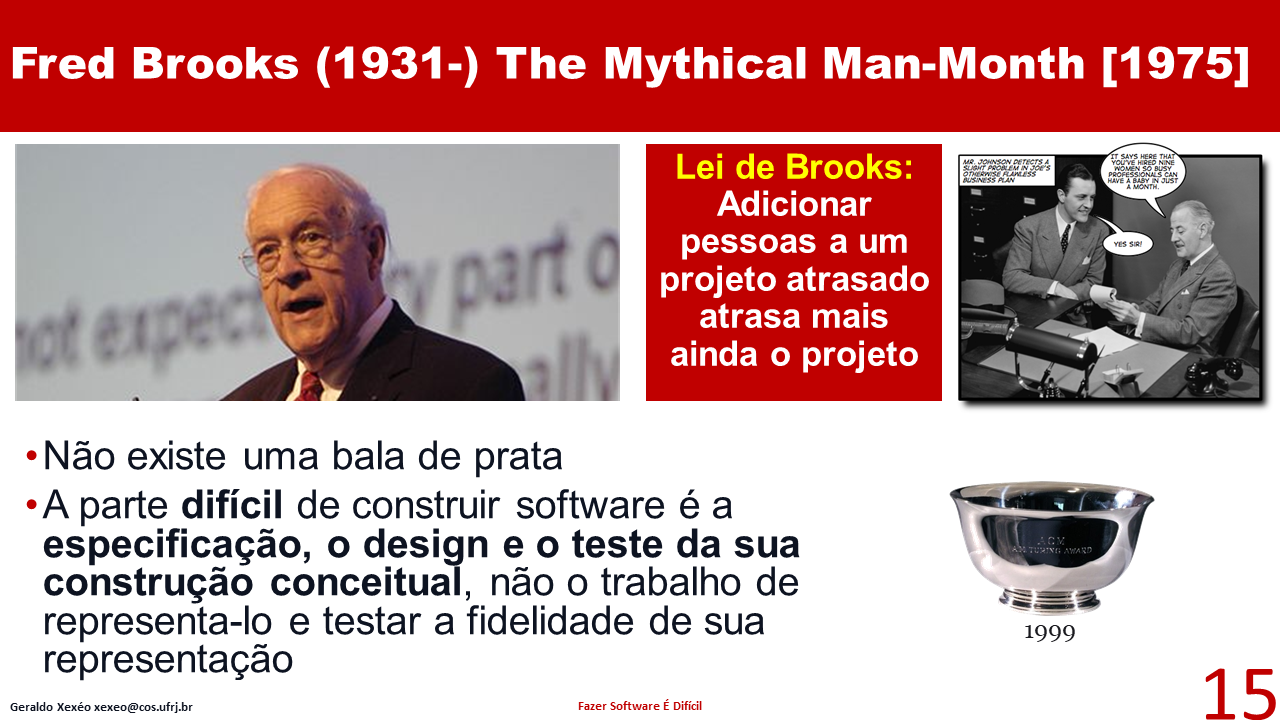
\includegraphics[width=\tam\linewidth]{imagens/manmonth.png}
    \caption{Um slide com um formato diferente}
    \label{fig:man}
\end{figure}


Os slides não devem ser exagerados, nem em texto, nem em decoração, porém um ou outro slide pode ser mais divertido, ou mais pesado em texto. Além disso, se todos os slides forem ``básicos'', parece que você não se esforçou para preparar a aula.

Em um slide com fórmulas, como o da Figura \ref{fig:formulas}, elas devem aparecer uma a uma se estiverem sendo calculadas.
Se for apenas um comentário sobre a complexidade das fórmulas, que você deseje passar por cima em busca de uma explicação mais fácil, elas podem aparecer todas de uma vez.

\begin{figure}[hbt]
    \centering
    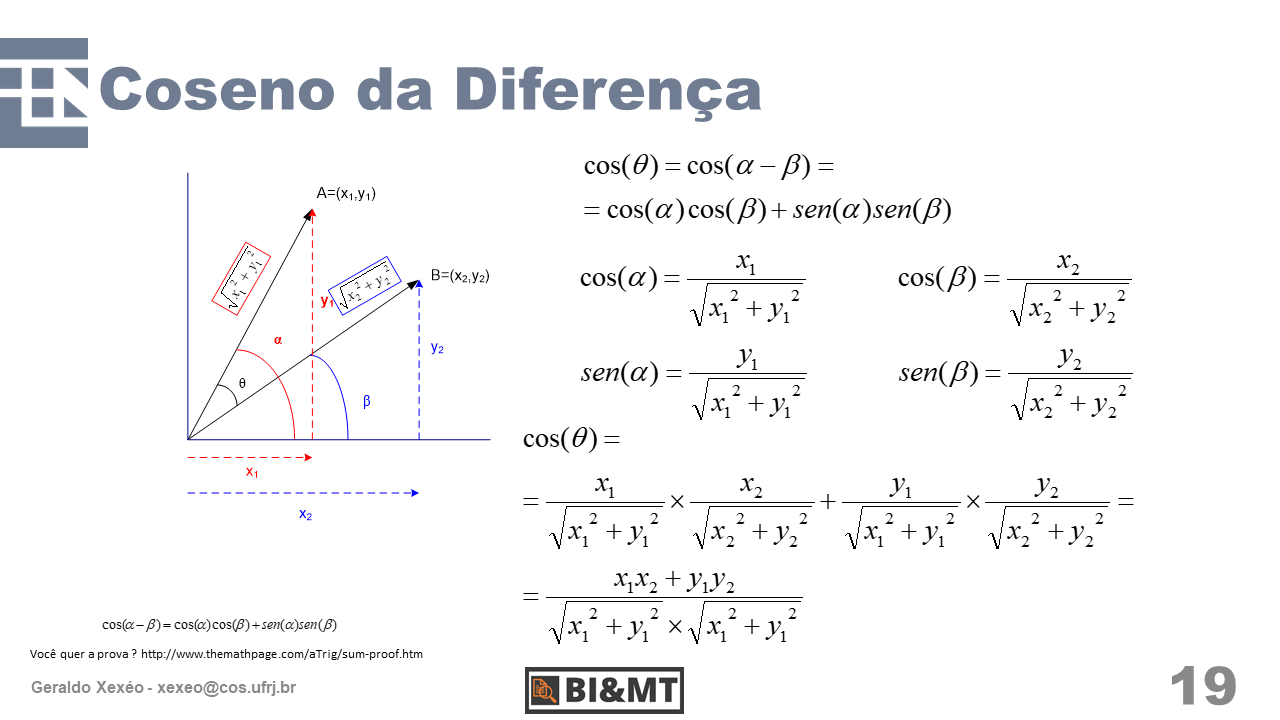
\includegraphics[width=\tam\linewidth]{imagens/desenhoeformulas.png}
    \caption{Desenho e fórmulas em um slide, que possui o logo do laboratório ligado ao curso e um logo que foi criado para identificar o curso em 3 lugares: Moodle, Whatsapp e GitHub.}
    \label{fig:formulas}
\end{figure}

\subsection{Que slides ter}

Os seguintes slides são recomendados para uma boa pontuação:
\begin{outline}
\1 Título da aula, como na Figura \ref{fig:titulo};
\2 Deve identificar candidato e ser feito como se fosse da instituição que faz o concurso;
\1 Objetivo da aula;
\1 Revisão do que é necessário para entender a aula;
\2 Contextualizando no curso
\1 Habilidades específicas que serão aprendidas;
\1 Agenda (ou Sumário);
\2 A agenda ou sumário divide a aula em seções;
\1 Um slide de título para cada seção;
\2 Pode ser o slide da agenda colocando ênfase na seção atual, como na Figura \ref{fig:meio};
\1 Slides de conteúdo;
\2 Não esqueça de uma motivação quando necessário;
\2 Não esqueça do contexto histórico do que está sendo ensinado;
\2 Não esqueça de definições
\1 Pelo menos um slide com um exercício
\2 Passar uma atividade de aprendizagem pós aula também é interessante, mesmo que ela nunca seja feita;
\1 Slide ``o que vimos hoje''
\2 Esse slide, ou slides, devem fechar a aula. Se necessário, por estar sobrando tempo, indique que agora, para reforçar, serão feitos ou discutidos exercícios, e siga por esse caminho até o fim do tempo;
\1 Referências bibliográficas;
\1 \textit{Preview} da próxima aula
\end{outline}

\begin{figure}[ht]
    \centering
    
\includegraphics[width=\tam\linewidth]{imagens/capa.png}
    \caption{Um slide de título.}
    \label{fig:titulo}
\end{figure}

Também é possível apresentar um slide de exercício no meio da aula. Nesse momento você deve ``quebrar a quarta parede'' e falar algo como ``normalmente eu daria 5 minutos e corrigiria o exercício, como vou fazer agora''.

Outra boa sugestão é ter um slide, no início, que leve a pensar sobre o conteúdo da aula. Esse slide pode mostrar um problema real onde a técnica poderia ser aplicada, sendo algo do tipo ``como vocês fariam para fazer x?''. Isso seria adequado para uma aula onde se ensina o método PERT/CPM para calcular prazos de um projeto. Já em uma aula de programação inicial, que vai usar exemplos numéricos, poderia ser proposto um problema numérico, como achar números primos.

Ao mostrar um problema é interessante mostrar como ele pode se complicar. Ao mostrar um método de fazer algo que suplantou outro anterior, é interessante mostrar os problemas que o anterior tinha. Deve haver cuidado, porém, na estimativa de tempo, o contexto histórico deve ser limitado a motivação. Se começar do início de tudo, você acabará tendo menos tempo para falar do assunto que deve abordar e poderá perder pontos.

\begin{figure}[hb]
    \centering
    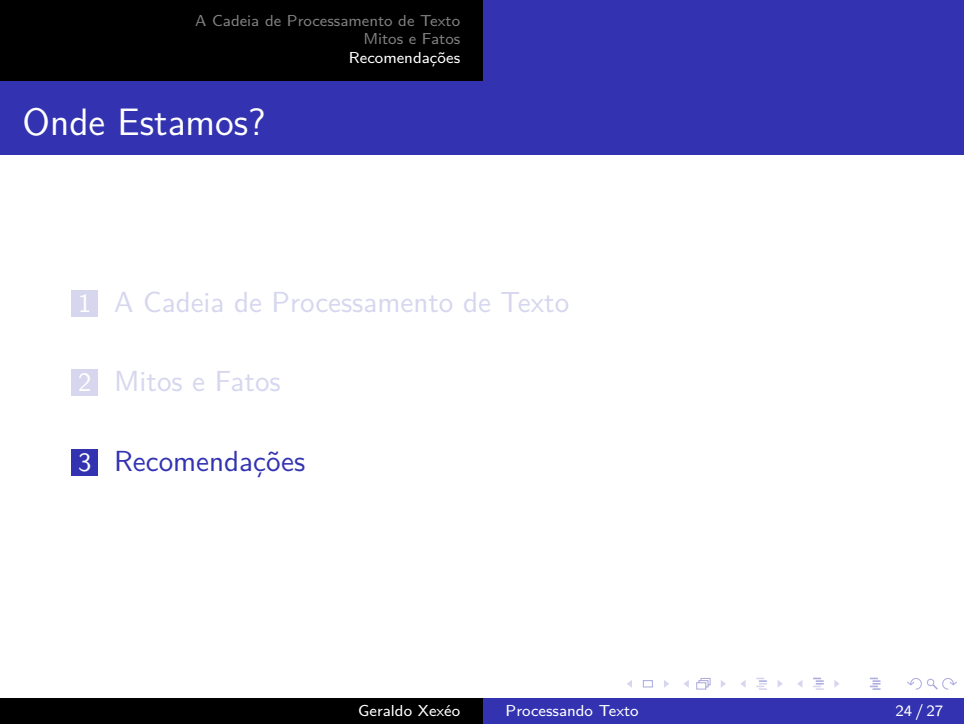
\includegraphics[width=\tam\linewidth]{imagens/agendadomeio.png}
    \caption{Um slide mostrando a parte que será falada da agenda, com as outras partes acinzentadas. Criada usando o \LaTeX\  e o \texttt{beamer}.}
    \label{fig:meio}
\end{figure}

Eu agora também crio mais um slide, que fala sobre a metodologia da aula, e o tamanho da aula em slides e em tempo, como na Figura \ref{fig:metodologia}.
Esse slide também mostra como símbolos podem ser usados para passar mensagens.
Julgo ser  uma boa ideia mostrar isso também, inclusive porque não é uma prática comum entre os professores e pode surpreender positivamente.

\begin{figure}[htb]
    \centering
    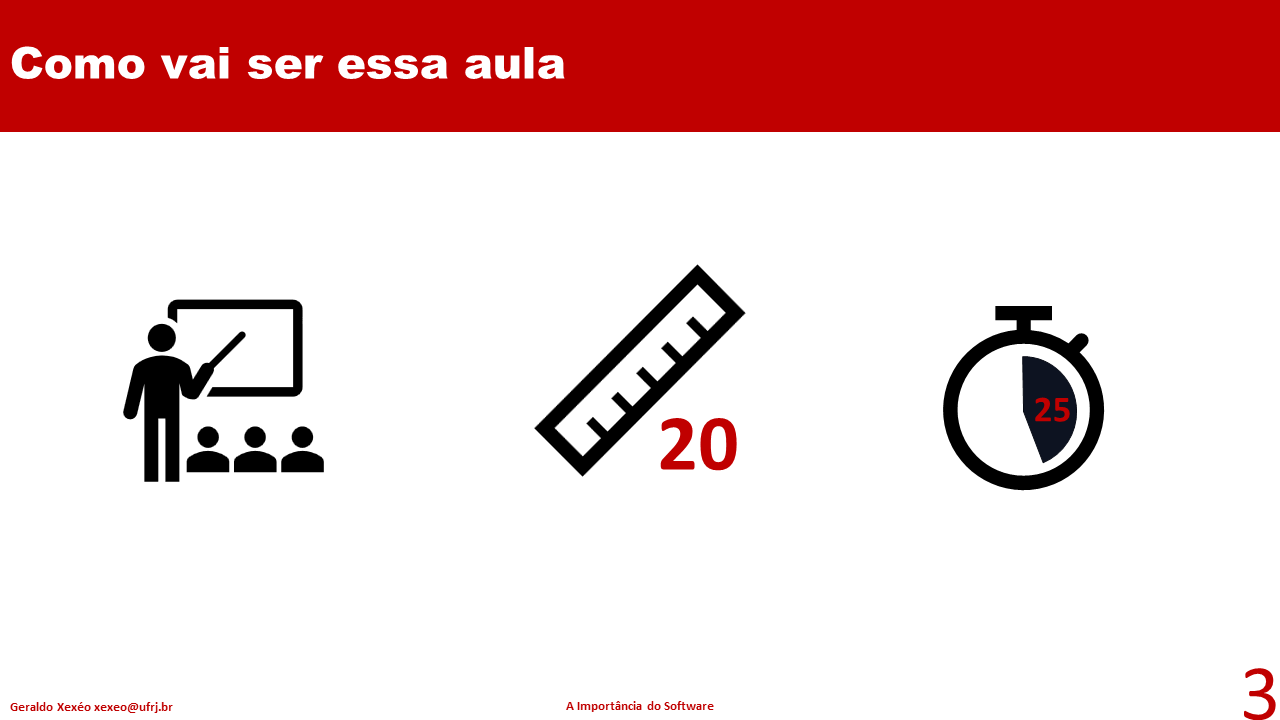
\includegraphics[width=\tam\linewidth]{imagens/metodologia.png}
    \caption{Slide informando o aluno como vai ser a aula.}
    \label{fig:metodologia}
\end{figure}


Em geral, qualquer prática didática adotada ativamente na aula vai ajudar a sua organização e, ao mesmo tempo, diminuir seu nervosismo.
Outra vantagem é que vai facilitar a compreensão da banca não só do que está acontecendo na sua aula, mas principalmente porque você escolheu dar a aula dessa forma.

Como adicional, um slide final sobre você. Hoje, todas as minhas aulas terminam com o slide da Figura \ref{fig:fim}.
Isso pode ser usado sempre para falar algo como ``quem quiser me contatar para tirar dúvidas...''.

\begin{figure}[hbt]
    \centering
    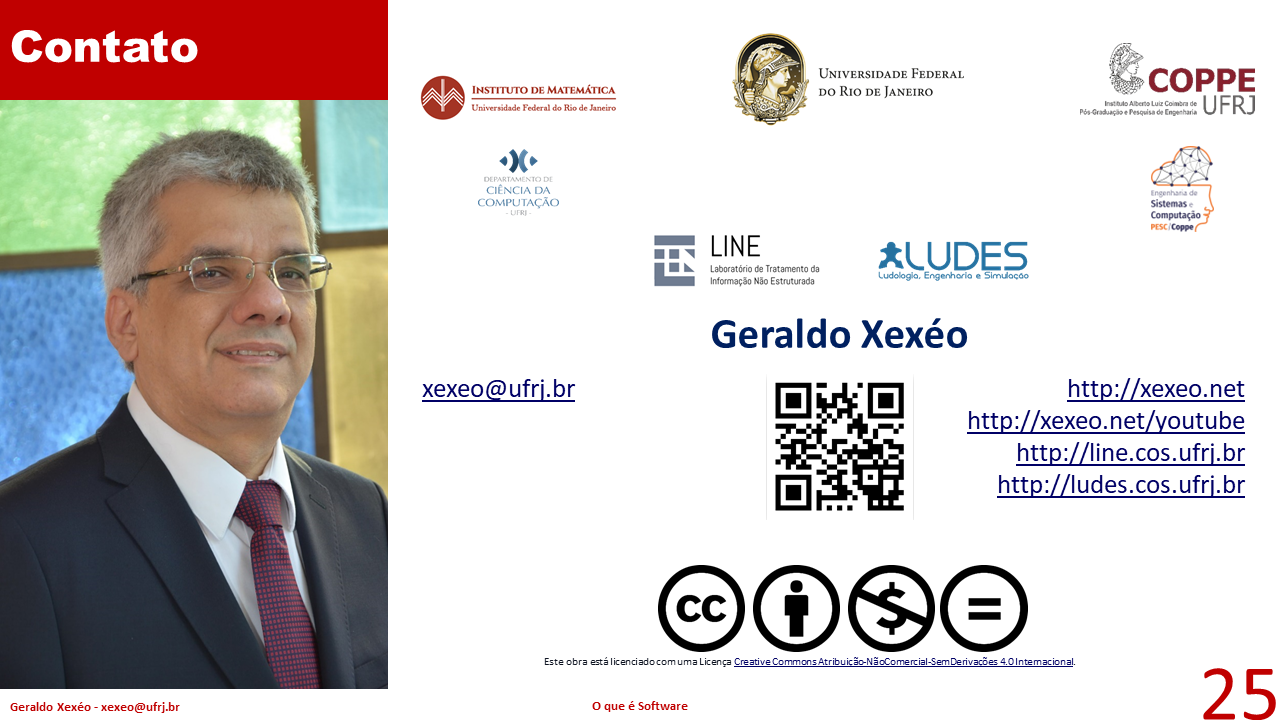
\includegraphics[width=\tam\linewidth]{imagens/fim.png}
    \caption{Um slide de contato.}
    \label{fig:fim}
\end{figure}

Forneça todas as referências, e indique a propriedade intelectual de tudo.
Prefira imagens de domínio público ou com licenças amplas, como \textit{Creative Commons}.

\subsubsection{O que não fazer}

Cuidado com dicas de como fazer slides de negócios, porque elas podem não se adequar ao que é esperado nos concursos.

Não use a técnica de uma grande imagem metafórica para grandes textos, porque é um material que não apoia o aluno.

\subsubsection{Storytelling}

Há uma nova tendência, porém, de usar \textit{storytelling}.
Uma aula bem dada pode usar a técnica de \textit{storytelling} em alguns casos.
Por exemplo, é possível dar uma aula de caso de uso a partir de um exemplo de modelagem de caso de uso onde os objetos do modelo vão aparecendo ao longo da história.

\subsection{Material adicional}

Você deve entregar para a banca, impresso, se possível, um material adicional. Normalmente esse material adicional não está descrito no edital, porém ele é parte esperada de uma aula. Os candidatos que entregam isso já partem com vantagem.

O principal material adicional que considero obrigatório é o \textbf{plano de aula}. Existem muitos modelos na Web, mas um bom plano inclui:
\begin{outline}
\1 pré-requisitos;
\1 conteúdo da aula;
\1 objetivos gerais e específicos da aula;
\1 habilidades que o aluno deverá adquirir;
\2 Se possível usando a taxonomia revisada de Bloom
\1 metodologia;
\1 recursos didáticos necessários;
\1 forma de avaliação, e
\1 referências.
\end{outline}

Outros materiais possíveis são:
\begin{outline}
\1 lista de exercícios;
\1 leituras adicionais, na forma de capítulos ou artigos;
\end{outline}

Além de entregar o material, você deve mostrar em um slide onde podem ser encontrados na rede, por exemplo em um Moodle, ou no GitHub.

Eu recomendo entregar pelo menos uma lista de exercícios além do plano de aula. O resto pode ficar referenciado no seu falso Moodle, e ser mostrado em um slide para a ``turma''.




\subsection{Dicas para a apresentação}

Como dito no início, a prova de aula é quase um teatro. Quanto mais próximo você for de uma aula bem dada, dentro de um contexto imaginário de um curso bem construído, mais pontos você fará. Além disso, se conseguir quem entre os candidatos e candidatas que apresentam o contexto de melhor forma, suas chances de estar no topo da classificação aumentam.

Durante a aula, a preocupação com o uso do português é essencial. Erros de português não só prejudicam a nota, mas também desviam a atenção da banca, tendo um efeito prejudicial duplo. Outro problema semelhante é o uso de cacoetes de linguagem, como as palavras tipo, coisa, expressões como ``se pá'', e o gerundismo. Uma aula com conteúdo brilhante pode ser considerada  uma prática medíocre em função dos defeitos de fala e apresentação que podem ser causados pela falta de experiência, por vícios de linguagem ou por nervosismo.

Treine a aula buscando principalmente fluência e ter a ideia correta do tempo. Não é necessário decorá-la. A intenção do treino é melhorar a sua fluência, dicção, perceber o que pode explicar a mais e a menos.

Eu acredito que a aula deve ser dada \textbf{realmente} como a pessoa daria para a turma, isso significa que pode fazer brincadeiras ocasionais e ser informal em parte da aula. Porém, como é, na verdade, uma banca, não deve exagerar nas brincadeiras ou fazer delas o tom da aula. É bom ter algumas brincadeiras preparadas. Uma dose de sinceridade também pode ser útil, como dizer que quando era aluno achava o assunto muito difícil e que tentaria ser mais claro para os alunos que seus professores foram para você.

É interessante introduzir curiosidades. Eu, por exemplo, ao dar a aula de Casos de Uso, sempre falo para que os alunos não desenhem o ator sendo assaltado, isto é, com os braços para cima. Também sempre cito se um autor de algo que estou apresentando ganhou algum prêmio por isso, principalmente o prêmio Turing.

Não dê a matéria sem contexto. Existem dois contextos, um é o do curso, fictício ou existente, onde cabe a aula. O candidato deve, por exemplo, mostrar algo que já foi ensinado e está sendo usado na aula que está sendo dada. O outro é o contexto da própria matéria. Quem criou, inventou, que prêmios ganhou, qual foi a motivação original, questões de mercado, qual a importância do assunto, onde é usado.

Procure pelo menos um exemplo real de uso, algo que possa contar, se possível, uma experiência pessoal.

\subsection{Como apresentar a aula}

Você deve falar sempre de frente e olhando para a banca, nunca falar de frente para os slides ou para o quadro, ou olhando para a tela do computador (veja a \autoref{fig:comparacao-apresentacoes}). Se tiver que usar o quadro, ou se virar, fale algo, então escreva ou desenhe de costas, em silêncio, e depois fale de novo.

\begin{figure}[hbt]
    \centering
    \begin{subfigure}[b]{0.45\textwidth}
        
\includegraphics[width=\linewidth]{dando aula.png}
        \caption{Posicionamento correto do candidato.}
        \label{fig:apresentacao-correta}
    \end{subfigure}
    \hfill
    \begin{subfigure}[b]{0.45\textwidth}
        
\includegraphics[width=\linewidth]{dando aula errado.png}
        \caption{Posicionamento indevido do candidato.}
        \label{fig:erro-apresentacao}
    \end{subfigure}
    \caption{Comparação entre uma apresentação correta e uma com erro.}
    \label{fig:comparacao-apresentacoes}
\end{figure}

No caso de aula remota, coloque a câmera sobre a tela onde estão as transparências.

Mantenha um ritmo de fala, fale para fora, de preferência mais alto, porém sem berrar. Professores sabem qual é o seu tom na aula e devem se aproveitar desse conhecimento.

Não se mexa muito, nem pouco, e use os movimentos a seu favor.  Use as mãos e braços para indicar e para fazer sinais que façam sentido na aula. Por exemplo, se estiver falando de uma mensagem passando de um lugar para o outro, pode fazer um movimento de transferência com as mãos. Não fique caminhando pela sala, a não ser que tenha um objetivo específico, como distribuir um exercício, e faça esforço para não cruzar na frente do projetor, criando sombras na tela.

Sei que esses conselhos são difíceis. Mas lembre-se, não adianta treinar para ser um robô. A banca procura professores que deem aula de maneira natural.


Não leia os slides. Eles devem ser uma referência de posicionamento e continuidade da aula. Eles sintetizam o que deve ser dito. Use figuras, mas não dê uma aula como as palestras ``da moda'', só com imagens inspiradoras do assunto, o slide deve conter informação para poder guiar uma revisão ou um estudo mais aprofundado.

Muito cuidado com posicionamentos ideológicos, e certamente não faça piadas ou comentários de qualquer cunho depreciativo, ou preconceituoso.


Se vai falar nome de pesquisadores estrangeiros, e deve fazê-lo para falar de autores, procure a pronúncia correta na rede. De forma aproximada, Djkstra se fala dáistra, Huizinga se fala Raizingá, Marie Curie se fala Marrí Currí. Se for muito difícil, ou incomum usarem o nome correto no Brasil, chame atenção ao fato como chamaria atenção de uma turma, diga que foi pesquisar, etc. Novamente, use curiosidades para tornar a aula mais interessante, como ``Aliás, o nome original de Marie Curie era Maria Salomea Sk\l odowska, pronunciado praticamente como se lê em português, como o ``w'' com som de ``v''''.

\subsection{Pecados}

Com o nervosismo, muitas vezes são cometidos alguns ``pecados'' que incomodam muito a banca, como:
\begin{outline}
\1 errar o português;
\1 pigarrear seguidamente para tentar limpar a voz, ou outras formas de limpar a garganta;
\2 leve uma garrafa de água para dar aula;
\3 cuidado para também não exagerar no tempo em que toma um gole ou na quantidade de água;
\1 repetir palavras, como ``ok'', ``tá'' a todo momento;
\1 tossir sem proteger a boca;
\2 proteja com o braço de preferência;
\2 no caso de aula remota por vídeo, desligue o microfone;
\1 se coçar demais, coçar o nariz, morder ou roer as unhas ao pensar;
\1 qualquer ato não higiênico ou mal educado em geral.
\end{outline}

A desorganização também é um ``pecado'' que é mal-visto pela banca. Você deve chegar pronto para a aula, deve conhecer o software que vai usar e, se possível, deve estar disponível no local antes do horário para preparar o seu material.





\subsubsection{Pecados do português}

A seguir apresentamos alguns exemplos de português que ``doem no ouvido'' da banca.
\begin{outline}
\1 Cuidado com o uso do verbo haver:
\2 Como em ``\textbf{Há} muitos anos, \textbf{havia} sardinhas na Baía da Guanabara''.
\1 Advérbios não variam em número ou gênero.
\2 ``As esposas estavam meio chateadas porque os maridos estavam meio bêbados''.
\1 Como sujeito de verbo se usa ``eu'' e nunca ``mim''. Para eu fazer, para eu comprar. Cuidado ao dizer ``para mim'' e depois  completar a ideia com verbo, o que leva ao erro.
\1 Cuidado com os cacófatos, como ``O menor nun\textbf{ca} \textbf{ga}nha do maior''
\end{outline}

\subsection{Considerações especiais}

É possível, e até importante,  examinar o material didático dos membros da banca. Deve se ter cuidado ao usar como referência ou pegar pedaços diretamente deles, e só fazê-lo se previamente autorizado, por condições do material, e fazendo a citação correta.

A aula propriamente dita deve ser toda sua. Você pode se inspirar para ver os tópicos que a banca acha importante na agenda, a bibliografia, e pode também usar imagens de livros que os professores da banca também usam. Ao fazer isso, porém, deve ter muito cuidado com o plágio.

\subsection{Regras mais importantes}

\begin{enumerate}
\item Use corretamente o português.
\item Pronuncie corretamente as palavras em outras línguas.
\item Verifique a correção e atualização do conteúdo da aula.
\item Organize-se.
\item Tenha atenção as práticas didáticas.
\item Treine para evitar o nervosismo.
\item Se divirta dando a aula.
\end{enumerate}

\section{Dicas para a Prova de Títulos}

Obtenha a planilha de cálculo para a prova de títulos e faça a sua avaliação dos pontos que fará.

Analise a planilha de cálculo e verifique seu currículo Lattes, que deve estar atualizado.

Prepare todas as documentações em uma pasta, ou várias, ordenadas na mesma ordem que a planilha, com seções com capas para as partes e linhas da planilha e com a indicação de quantos documentos estão sendo apresentados.

Se possível, marque com algum \textit{tag} as seções e subseções da sua pasta de comprovação de títulos.  Por exemplo com \textit{post-its} marcadores de página identificados com os números das seções.

Também é possível encadernar as comprovações da prova de títulos, por exemplo com encadernação espiral, em vez de colocá-los em pastas.

\section{Colabore!}

Este texto foi escrito como uma conversa com uma pessoa da qual não é necessário conhecer o gênero. Esta pessoa é chamada de você, como se faz no Rio de Janeiro. Ele foi revisado para ser indiferente ao gênero de todas as formas possíveis quando lido, não fazendo também suposições sobre o gênero da pessoa que se candidata à vaga. Se você julga que em alguma parte do texto esta intenção se perde, por favor se comunique comigo.

Se você tem outras dicas, por favor mande uma mensagem para mim.

\section{Licença}

Este texto é distribuído com uma licença Creative Commons - Atribuição - NãoComercial - Compartilha Igual 4.0 Internacional.


Você tem o direito de:
\begin{itemize}
\item \textbf{Compartilhar} -- copiar e distribuir o material em qualquer suporte ou formato.
\item \textbf{Adaptar} -- remixar, transformar, e criar a partir do material.
\end{itemize}

De acordo com os termos seguintes:
\begin{itemize}
\item \textbf{Atribuição} -- Você deve dar o crédito apropriado, prover um link para a licença e indicar se mudanças foram feitas. Você deve fazê-lo em qualquer circunstância razoável, mas de nenhuma maneira que sugira que o licenciante apoia você ou o seu uso.
\item \textbf{NãoComercial} --Você não pode usar o material para fins comerciais.
\item \textbf{CompartilhaIgual} -- Se você remixar, transformar, ou criar a partir do material, tem de distribuir as suas contribuições sob a mesma licença que o original.
\item \textbf{Sem restrições adicionais} -- Você não pode aplicar termos jurídicos ou medidas de caráter tecnológico que restrinjam legalmente outros de fazerem algo que a licença permita.
\end{itemize}

Mais informações podem ser encontradas em \url{https://creativecommons.org/licenses/by-nc-sa/4.0/deed.pt_BR}
\end{document}
